% Appendix C

\chapter{Damage Equivalent Load (DEL) Calculation} % Main appendix title

\label{AppendixC} % For referencing this appendix elsewhere, use \ref{AppendixA}

\lhead{Appendix C. \emph{Damage Equivalent Load (DEL) Calculation}} % Change X to a consecutive letter; this is for the header on each page - perhaps a shortened title

Damage equivalent loads are calculated by MLife, A fatigue analysis tool developed by NREL \cite{hayman2012,hayman2012a}. MLife automates the damage analysis techniques outlined in Annex G of IEC 61400-1 \cite{IEC2005}. The load history of a component, as shown in Figure \ref{figC-1} , can be thought of as a series of load cycles. Each of those load cycles has some mean load and cyclic loading range. If damage accumulates linearly and independently for each cycle, as proposed by Palmgren \cite{palmgren1924} and Miner\cite{miner1945}, then the total damage from all cycles will be given by:

\begin{equation}
D_{fatigue} = \sum_{i} \frac{1}{N_{fatigue, i}} \label{eqC-1}
\end{equation}

 \begin{figure}[ht]
	\centering
		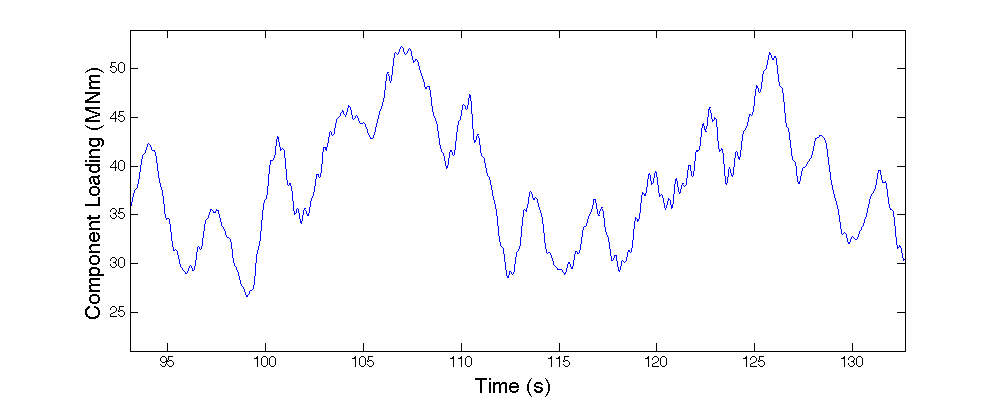
\includegraphics[width=\linewidth]{Figures/AppendixCFigures/figC-1.png}
	\caption{Example of component loading.}
	\label{figC-1}
\end{figure}



where $N_{fatigue, i}$ denotes the number of cycles to failure for the $i^th$ loading cycle. For example, if the $i^th$ loading cycle would have to be repeated 10,000 times to drive a new component ($D_{fatigue} = 0$) to failure ($D_{fatigue} = 1$) then $N_{fatigue, i} = 10,000$ and the damage accumulated due to the $i^th$ loading cycle would be 0.0001. For a given loading cycle $N_{fatigue, i}$ is estimated by:

\begin{equation}
N_{fatigue, i} = \left ( \frac{L_{ultimate}-L_{mean}}{\frac{1}{2}L_{range,i}} \right )^m \label{eqC-2}
\end{equation}

where $L_{ultimate}$ is the ultimate design load of the component, $L_{mean}$ is the mean load over the component's load history, $L_{range,i}$ is the $i^{th}$ cycles range, and m is the W\"{o}hler exponent. It can be seen in equation \ref{eqC-2} that larger loads cause more damage. Increasing the load cycle range or the mean load lead to smaller values of $N_{fatigue, i}$, which means more damage per cycle.  

The W\"{o}hler exponent is a property of the component under consideration, but it is highly dependent on the material the component is made from. For damage equivalent load calculations in this dissertation m was assumed to be 10 for steel components (tower) and 4 for fiberglass components (blades). These are the values of m that Stewart, Lackner, Haid, Matha, Jonkman, and Robertson used to perform fatigue analysis of the NREL 5 MW turbine in \cite{stewart2013}.

Because the NREL 5MW turbine is a fictional turbine ultimate loads ($L_{ultimate}$) are not available for it's components. This presents a problem when attempting to calculate accurate fatigue damage ($D_{fatigue}$) estimates. However, this problem can be circumvented if we use the component load history to calculate a damage equivalent load instead of using it to calculate fatigue damage. 

The damage equivalent load (DEL) is a constant amplitude fatigue load that occurs at a fixed frequency and produces the same damage as the actual load history of the component. The damage caused by the DEL is:

\begin{equation}
D_{fatigue} =  \frac{n_{equivalent}}{N_{equivalent}} \label{eqC-3}
\end{equation}

\begin{equation}
N_{equivalent} = \left ( \frac{L_{ultimate}-L_{mean}}{\frac{1}{2}DEL} \right ) \label{eqC-4}
\end{equation}

where $N_{equivalent}$ is the number of cycles to failure for the damage equivalent load, and $n_{equivalent}$ is the number of damage equivalent loading cycles the component is subjected to. $n_{equivalent}$ is chosen by the analyst. All DEL calculations in this dissertation have used $n_{equivalent} = 1$. In other words, the complex load history of the components under consideration have been converted to single loading cycles that cause equivalent damage. Setting $n_{equivalent} = 1$ and combining equations \ref{eqC-1} and \ref{eqC-3} yields:

\begin{equation}
\sum \frac{1}{N_{fatigue, i}} = \frac{1}{N_{equivalent}} \label{eqC-5}
\end{equation}

Substituting in equations \ref{eqC-2} and \ref{eqC-4} then solving for DEL gives:

\begin{equation}
DEL = \left ( \sum_{i} \left ( L_{range,i} \right )^m \right )^{\frac{1}{m}} \label{eqC-6}
\end{equation}

We see from equation \ref{eqC-6} that the ultimate load of the component is not required to calculate the damage equivalent load. the DEL does quantify the amount of damage done to a component, but it is a useful tool for comaring the relative damage done by two time histories. A higher DEL indicates more damage. In this dissertation DEL is used to compare various control strategies to see if they reduce or increase the damage experienced by the turbine.

A few notes on the Goodman correction: The DEL calculations carried out in this dissertation, as outlined above, do not include the Goodman correction. When the Goodman correction is used, equation \ref{eqC-2} becomes:

\begin{equation}
N_{fatigue, i} = \left ( \frac{L_{ultimate}-L_{mean,i}}{\frac{1}{2}L_{range,i}} \right )^m \label{eqC-7}
\end{equation}

where $L_{mean,i}$ is the mean load for the $i^{th}$ loading cycle, not the mean load of the load history. Using the Goodman correction leads to more accurate estimates of fatigue damage. However, when the goodman correction is used, the equation for DEL is not independent of the ultimate load:

\begin{equation}
DEL = \left ( \sum_{i} \left ( L_{range,i}\left ( \frac{L_{ultimate}-L_{mean}}{L_{ultimate}-L_{mean},i} \right ) \right )^m \right )^{\frac{1}{m}} \label{eqC-8}
\end{equation}

Since accurate estimates of $L_{ultimate}$ were not available for NREL 5 MW components, the Goodman correction was not used for DEL calculations in this dissertation.